\definecolor{gray}{gray}{0.6}
\section{Sprint 2}

\subsection{Sprint planning}
	In this sprint, the group is planning on a big delivery. In last sprint the group
	implemented the fundamental structure in the game as models, presenters and views. 
	The implementations in the last sprint was crucial for this sprint in order to 
	be able to implement a lot of game logic to make the game "playable".

	The group will focus on the requirements with critical and high priority in order
	to deliver as promised. There will also be more focus on the implementation, rather
	than writing more content to the report.

	When the group is in the end of this sprint, we will also use time on the testing.
	The tests is from the testplan and will enusre that the product that is made
	as we have planned and that the product works before the sprint delivery with the customer. 
	The testing is manually because we will not be able to implement unit test becuse
	there is not time for that in this sprint.

	During this sprint, the group needs to focus more on the workload becuase we did
	not manage to reach the worklad expected from the course staff. This is crucial
	for the group in order to be able to deliver the product and meet the deadlines.

\subsection{Expected sprint results}
	In this sprint the group will focus on the implementation and will try to deliver
	as much functionality as we can. In the last sprint, the group focused on the report and creating
	the base for future implementations	and not that much on the implementation of the 
	functional requirements. 

	The goal for this sprint is to implement as much as we can of the critical and 
	high requirements as we can in order to deliver a "playable" game in the sprint delivery.
	This is a high priority because the customer have not get the opportunity to 
	play the game yet. 
	In the end of this sprint, there should not be many unimplemented critical and high 
	priority requirements left. 

\subsection{Duration and worklaod}
	In the last sprint, we did not reach the workload expected by the course staff.
	In the start of the sprint, the scrum master made timetable together with the
	scrum team in order to ensure more workload. The goal was to at least have an
	avrage workload pr/person to be 25 hours pr/week. 

	{\bf Duration:} 30.09 - 13.10 (2 weeks)\\
	{\bf Workload:} This is the list with hours spent (the whole grup) on the project in this sprint.
	\begin{itemize}
		\item {\bf Planning:} 11 hours
		\item {\bf Development:} 85 hours
		\item {\bf Design:} 0 hours
		\item {\bf Documentation (report):} 65 hours
		\item {\bf Testing:} 3.5 hours
	\end{itemize}
	{\bf Total workload: } 165 hours \\

	The group's goal was to work at least 20-25 hours pr/person every week in this sprint. 
	We did manage the workload, and we had a avrage of 20.6 hours/week (165 hours/4 persons/2 weeks = 20.6 hours). 
	The scrum master have the responsability to ensure that the worklad is met with the
	expectations from the course staff, and we managed it in this sprint.
	The changes from the last sprint is that we worked late hours and used the weekend effective
	since alle the group members are occupied with UKA, vulentary work and homework.

\subsection{Sprint backlog}

	In this sprint we planned to implement the most of the requirements with critcal and high
	priority. In the start of the sprint we only planned to implement 8 requirement, but
	during the sprint we manage to implemet them and added more requirements to the sprint backlog.
	In the end of the sprint the backlog consisted of a total of 15 requirements. Here are the
	sprint backlog from this sprint:

	\begin{tabular}{| p{1cm} | p{8cm} | p{3cm} |}
		\hline
		\rowcolor{gray}
		ID & Description & Estimate \\ \hline
		FR1.1 & The user should be able to read game instructions from the main menu
		& \\ \hline

		FR1.12 & The user should not get the opportunity to tilt the screen by tilting the phone. & \\ \hline
		
		FR2.2 & The user should be able to buy and place several power stations on the game map.
		& \\ \hline

		FR2.3 & The user should be able to buy and place power cables on the map. &  \\ \hline

		FR2.4 & The user should be able to upgrade the powerplant. & \\ \hline

		FR2.8 & The user should be able to see information about a buildings when tapping on them.
		& \\ \hline

		FR3.6 & When an existing building is not supplied with power within a certain amount of time, 
		the house should dissapear and the player's health score should decrease. & \\ \hline

		FR4.2 & The user should be able to continue a level while the health score is greater than zero. 
		When the health score reaches zero, the game is over. & \\ \hline

		FR5.1 & The user should be able to collect money from the buildings connected to the power plant
		& \\ \hline

		FR5.2 & When connecting buildings through power cables, there should be a cost which is 
		proportional to the length of the cable. & \\ \hline

		FR5.3 & It should cost money to upgrade the powerplant. & \\ \hline

		FR6.3 & The user should be able to click on a power plant to receive information about 
		the cost of upgrading it and what the upgrade does. & \\ \hline

		FR6.7 & The user should be able to see the main menu when he/she starts the game. & \\ \hline

		FR6.8 & When the player wants to place a powerplant or a power cable in building mode, 
		the player should be prompted if they want to go through with it, or cancel. & \\ \hline

		FR6.9 & The user should be able to see that he/she is in building mode when selecting 
		a building to build in the hub menu. & \\ \hline

		FR6.10 & The user should be able to see that a building has gone without power for 
		some time, and is affecting the player's health score if the building is not connected 
		to a powerplant before it dissapears. & \\ \hline

	\end{tabular}

\subsection{Implementation}
	
	This is the actual implementation of requirements that we managed to implement
	from the sprint backlog.
	
	\begin{itemize}
		\item {\bf Building mode:} When the player open the hud (menu in the buttom of the screen) and presses
		on the build powerplant/powercable image, the player enters the building state 
		"build powerplant/build powerlines". The game state is set back to normal after the player 
		is finished whith the building. The game has a state variable that contains whitch mode the 
		game is in (Normal, build powerplant or build powerlines). When the player is in the building
		state, two lines will appear (on top and buttom) on the screen that looks like custruction mode
		(yellow and black stripes). The look and feel is important for the user to uderstand that
		the gamestate is changes to building mode. 

		\item {\bf Upgrade powerplants:} When the player taps on the powerplant, a pop-up will appear.
		In the pop-up it will show the level the powerplant is in and how much it will cost the 
		player to upgrade the powerplant. If the player choose to upgrde the powerplant the level will
		increase by 1. If the player do not want to upgarde, he/she press "cancel" and the player will be sent
		back to the game. The part that is not implemented here is that when a powerplant is upgarded, 
		it will be able to serve more buildings with power and this should also be added to the building 
		information in the pop-up. If the player does not have enough money, the player gets a message 
		that he/she cannot upgarde.

		\item {\bf Building and buy powerplants:} When the player open the menu in the bottom and 
		choose the "build powerplant" icon, the player enters the building mode and is able to 
		tap on the screen where he/she wants to place the powerplant. When the player taps on the
		location to place the building, it will a apperar a pop-up with the question if the player 
		want to buy and build the powerplant. If the player want to build the powerplant, a certain
		amount of money will be payed from the players money or if the player press "cancel", the 
		game goes out of the building state and back to normal. If the player choose to buy the 
		powerplant, but do not have enough money, the player get a message that he/she do not have
		enough money and the game state will be set back to normal. 

		\item {\bf Connect buildings to powerplants:} When the player open the menu in the bottom and 
		choose the "build powerline" icon, the player enters the building mode and the player is able
		to build powerlines. The powerlines is build by tapping on the desired en-points (house-house 
		or house-powerplant).

		The part that is not implemented is the logic for handling the "connection state" of a building, 
		as well as the amount of power a powerplant can serve. It is not implemented that if the building
		is connected, the countdown will stop and make money that the player can collect. The money should
		only be "produced" if the building is connected to a powerplant. The amount of money that is 
		produced should be building specific becuase different buildings use different amount of power, and
		therefore need to pay a different amount of money. 

		\item {\bf Collect money:} When a building is connected to another building, it starts 
		"producing" money. The building will show a icon of a coin when the player is able to 
		collect the money. The money is collected when the user taps on the building with a coin. 

		The parts that is missing is that it needs to check wheter the connected builing is a powerplant 
		or just another building. It should only produce money if it is connected to a powerplant. 
		If the building have produced money, a coin will appear on the building. When the player tap
		on a building with a coin icon, it will collect the money and the players amount of money 
		will increase. 

		\item {\bf Game over:} When the healthbar is zero, the game is over and the game over screen 
		is showing. When the player press "ok", the player is sent to the main menu and is able to 
		start a new game. This part may need som changes to the look and feel, but it is working.

		\item {\bf Main menu:} When the game is starting, the app is showing the main menu. 
		From this menu, the player is able to choose between "Start game", "Instructions" and highscore.

		\item {\bf Money and goal:} When the player has started the game, the score and goal for
		the levl is showing in the hud. To get to the next level, the player need to get the same
		amount of money as the goal in order to go to the next level. The logic for the level
		is not finished yet.

		\item {\bf Information about powerplant:} If the user taps on a powerplant it will pop up
		information about the powerplant like level and upgradeinformation. It is not implemented yet,
		but it will be implemented more information like how much power it can serve and how mange
		buildings that are connected. 

		\item {\bf Healthbar:} In the bottom of the game it is showing a healthbar. If the 
		healthbar is below zero, it is game over, so the player need to keep track of the health.
		A user loses helath if a new buildings countdown is over and the buildning dissapears.
		The healthbar will send a singnal with a color. If the player has full healthbar the bar is
		green, then it gets orange and in the end it is red. 

		\item {\bf Countdown on building:} when a building appear, a countdown starts. If the player
		do not connect the building to a powerplant, the countdown wont stop. If the countdown is
		finished, the house will dissappear and the healthbar will decrease. This is a signal to
		the player so he/she is able to connect the building to a powerplant in order to not loose
		health. 

	\end{itemize}

	This is the requirements that was in the sprint backlog that we did not
	manage to finish and have removed to sprint 3:

	\begin{itemize}
		\item {\bf Information about building:}

		\item {\bf The cost of the powerlines:}

	\end{itemize}

	\begin{figure}[H]
	\centering
	\subfigure{
		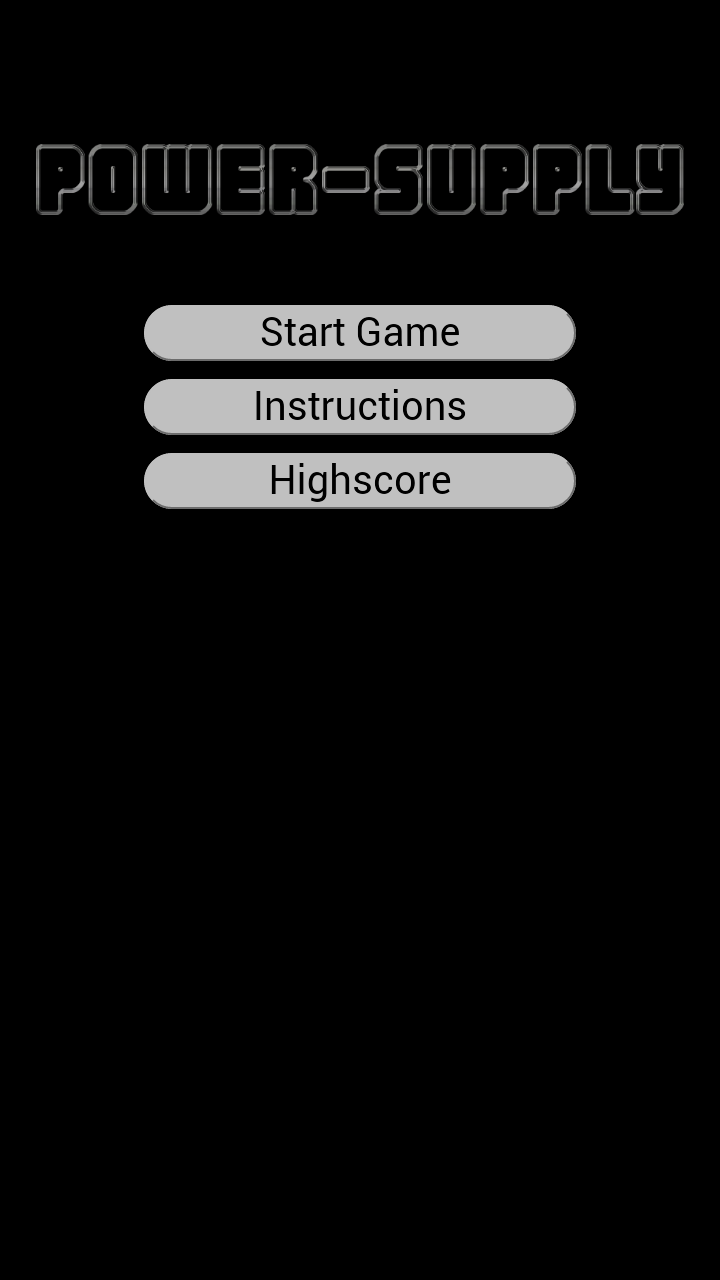
\includegraphics[scale=0.17]{pictures/sprint2-screen/sprint2-2}
	}
	\subfigure{
		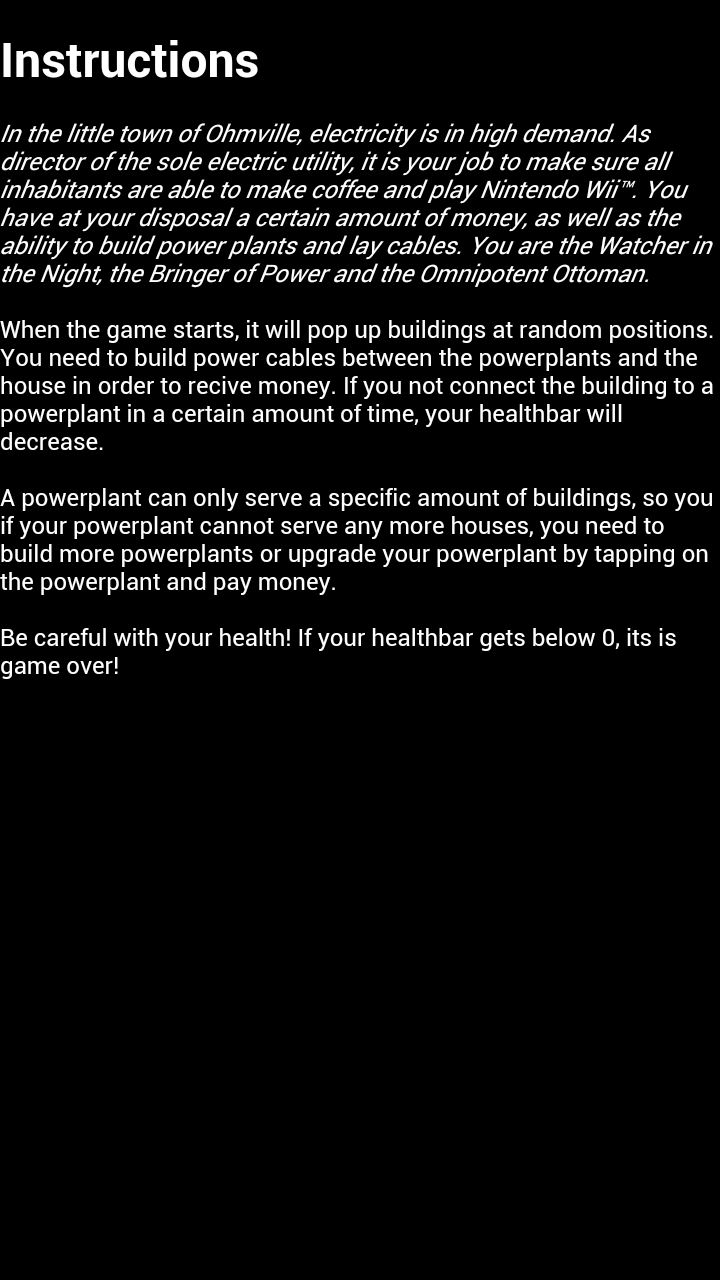
\includegraphics[scale=0.17]{pictures/sprint2-screen/sprint2-3}
	}
	\caption{This is blabla}
	\end{figure}

	\begin{figure}[H]
	\centering
	\subfigure{
		
\includegraphics[scale=0.17]{pictures/sprint2-screen/sprint2-4}
	}
	\subfigure{
		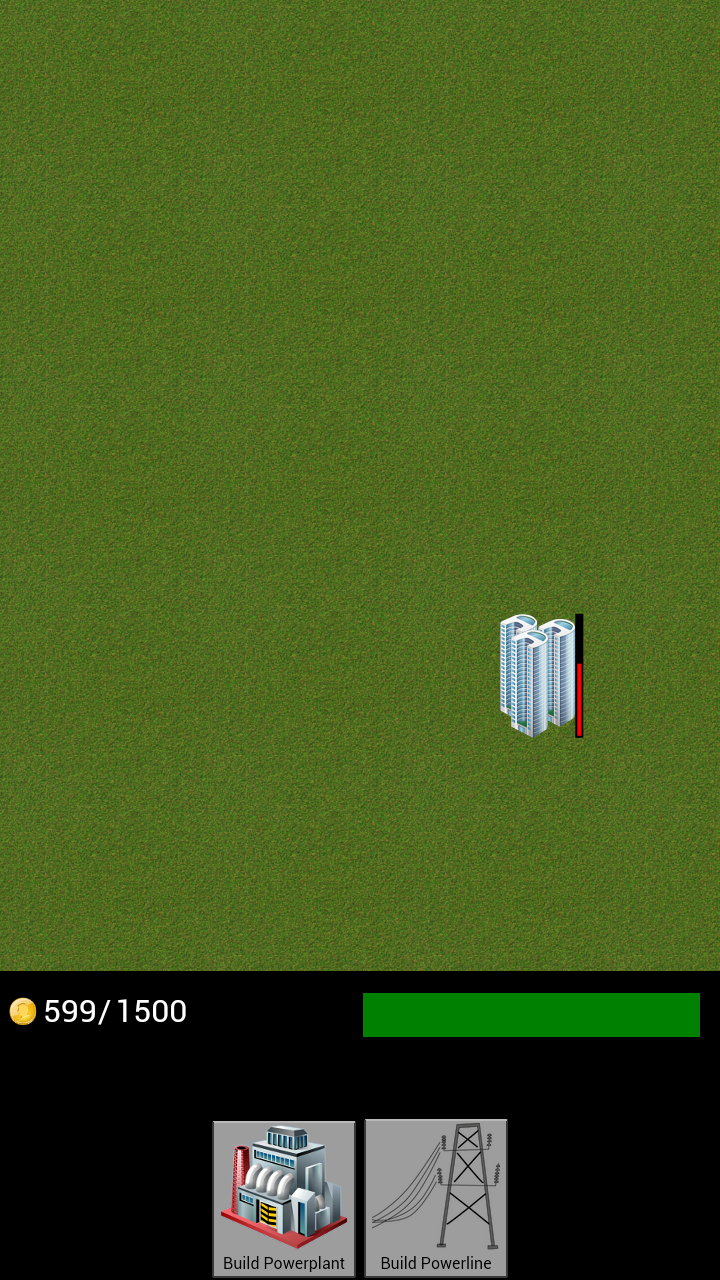
\includegraphics[scale=0.17]{pictures/sprint2-screen/sprint2-5}
	}
	\caption{This is blabla}
	\end{figure}

		\begin{figure}[H]
	\centering
	\subfigure{
		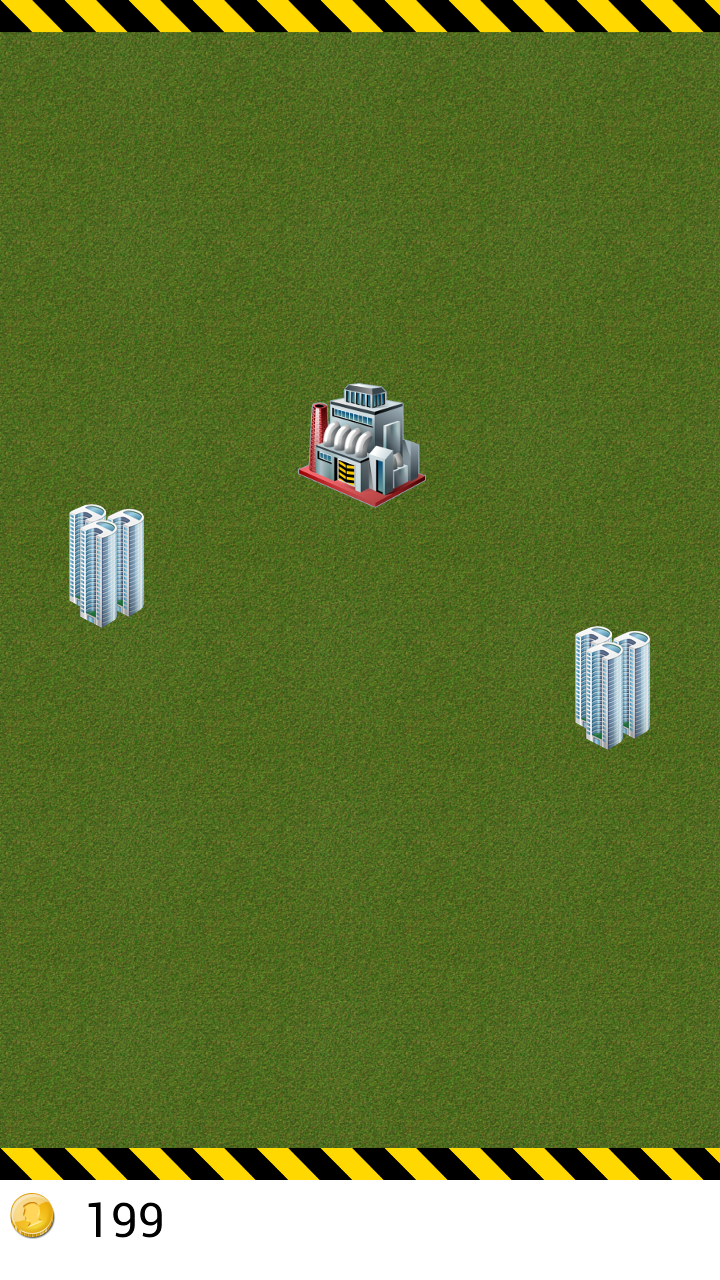
\includegraphics[scale=0.17]{pictures/sprint2-screen/sprint2-1}
	}
	\subfigure{
		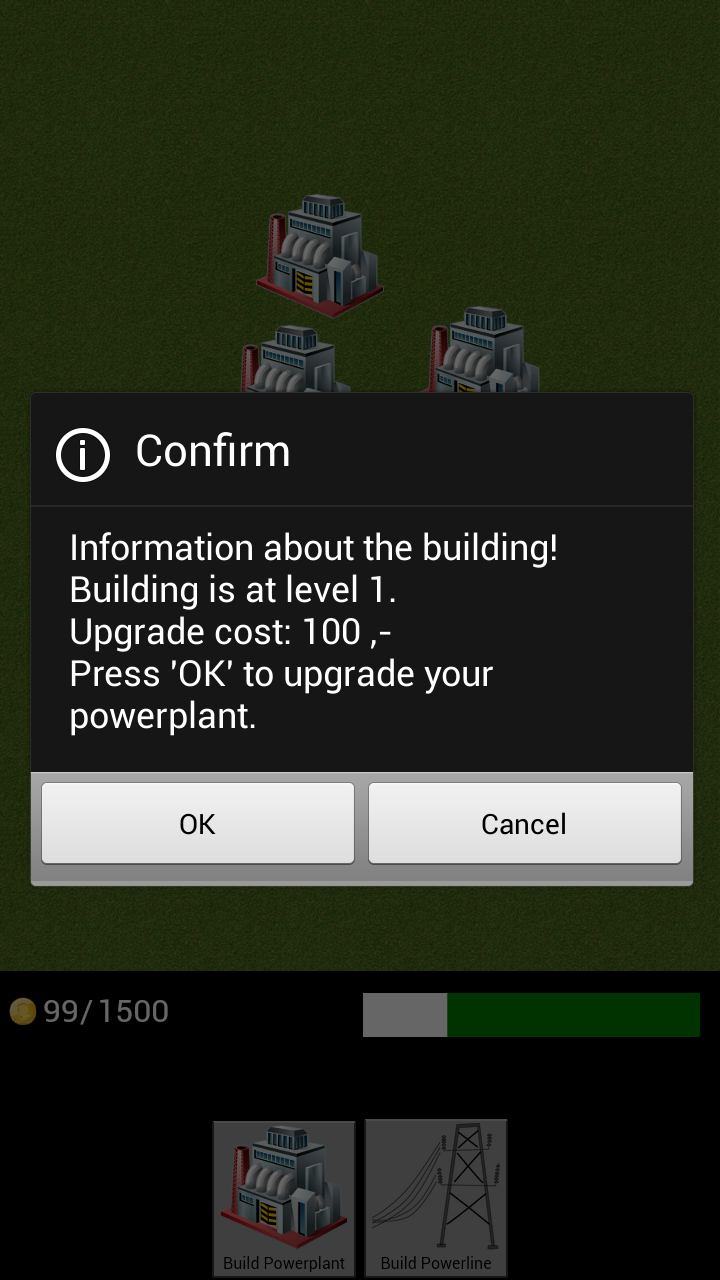
\includegraphics[scale=0.17]{pictures/sprint2-screen/sprint2-12}
	}
	\caption{This is blabla}
	\end{figure}

	\begin{figure}[H]
	\centering
	\subfigure{
		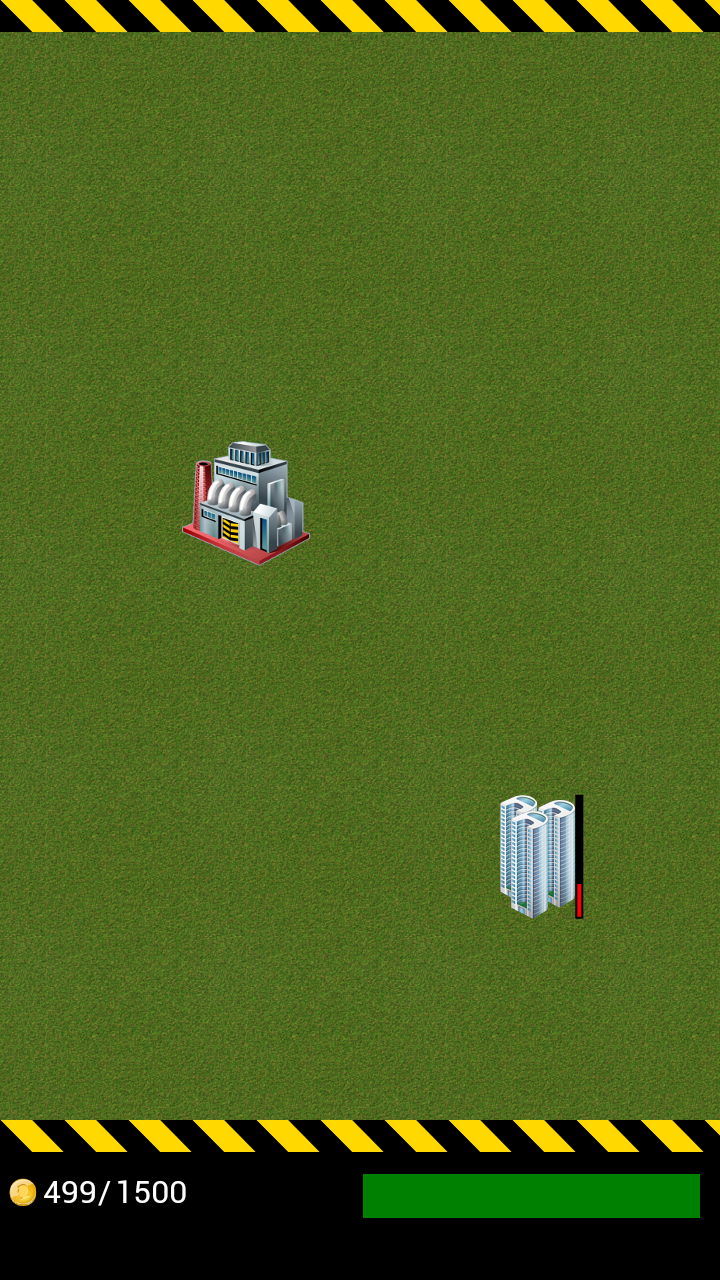
\includegraphics[scale=0.17]{pictures/sprint2-screen/sprint2-6}
	}
	\subfigure{
		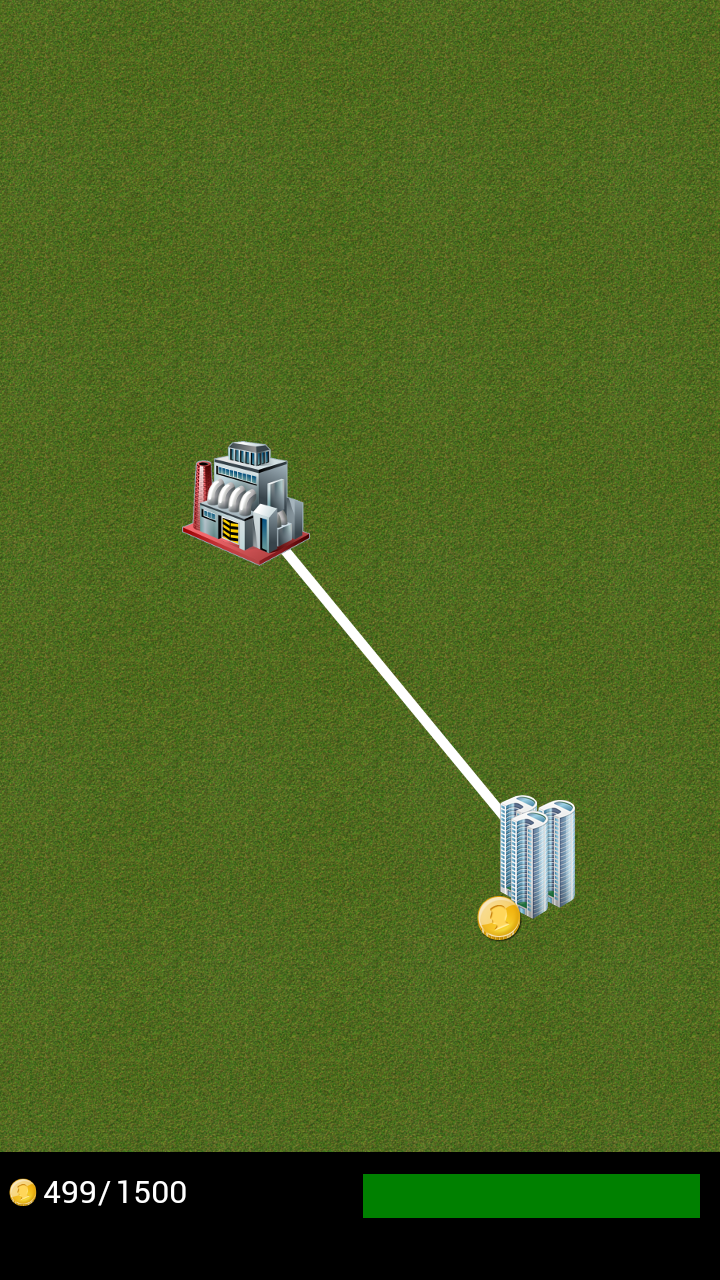
\includegraphics[scale=0.17]{pictures/sprint2-screen/sprint2-7}
	}
	\caption{This is blabla}
	\end{figure}

		\begin{figure}[H]
	\centering
	\subfigure{
		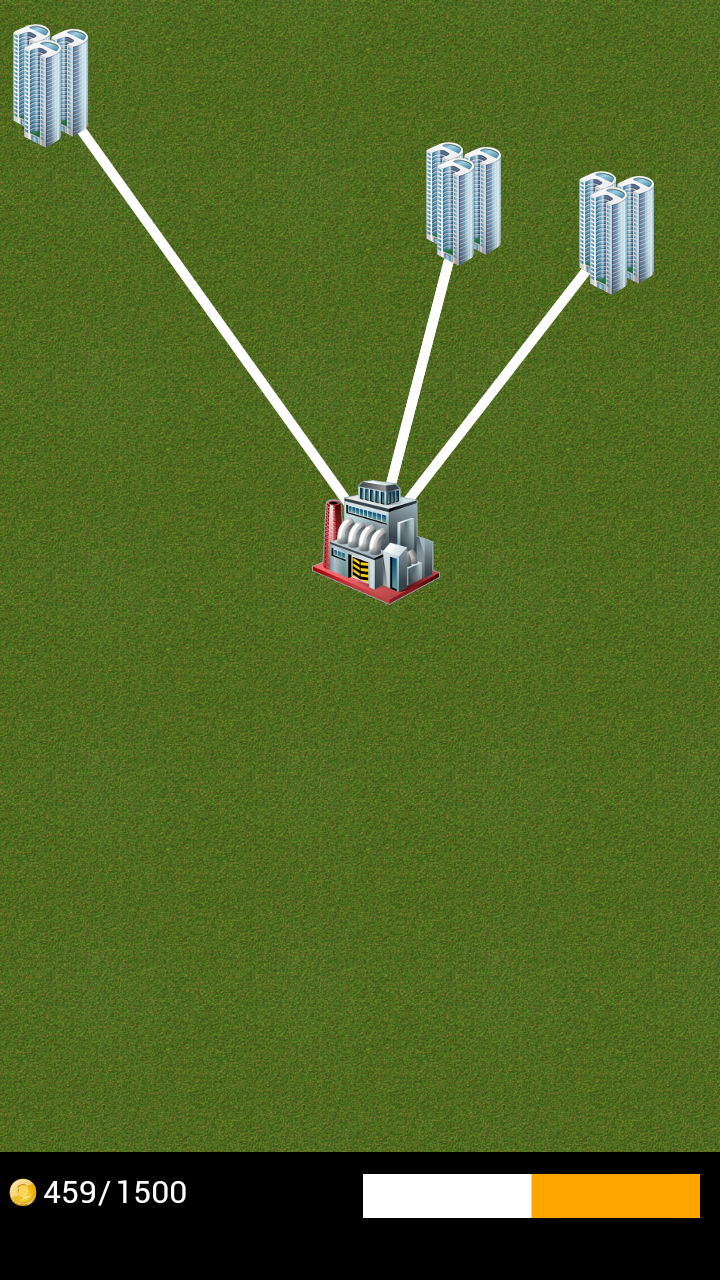
\includegraphics[scale=0.17]{pictures/sprint2-screen/sprint2-8}
	}
	\subfigure{
		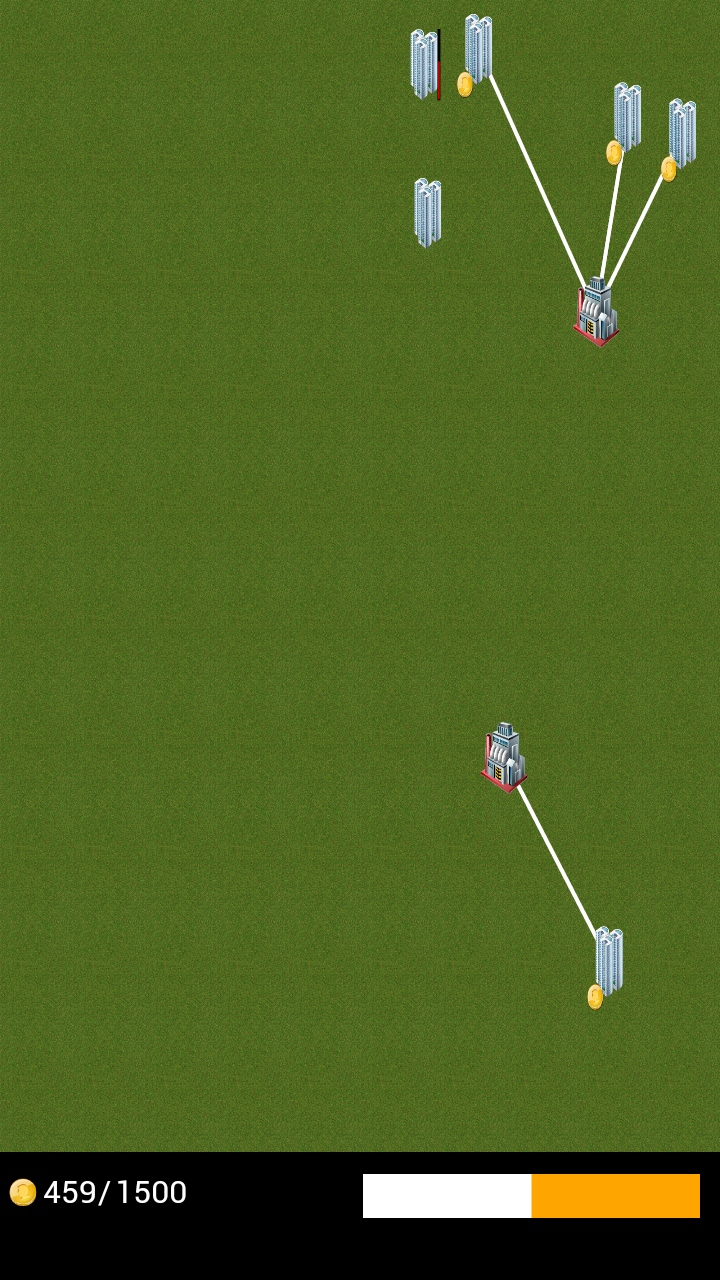
\includegraphics[scale=0.17]{pictures/sprint2-screen/sprint2-9}
	}
	\caption{This is blabla}
	\end{figure}

	\begin{figure}[H]
	\centering
	\subfigure{
		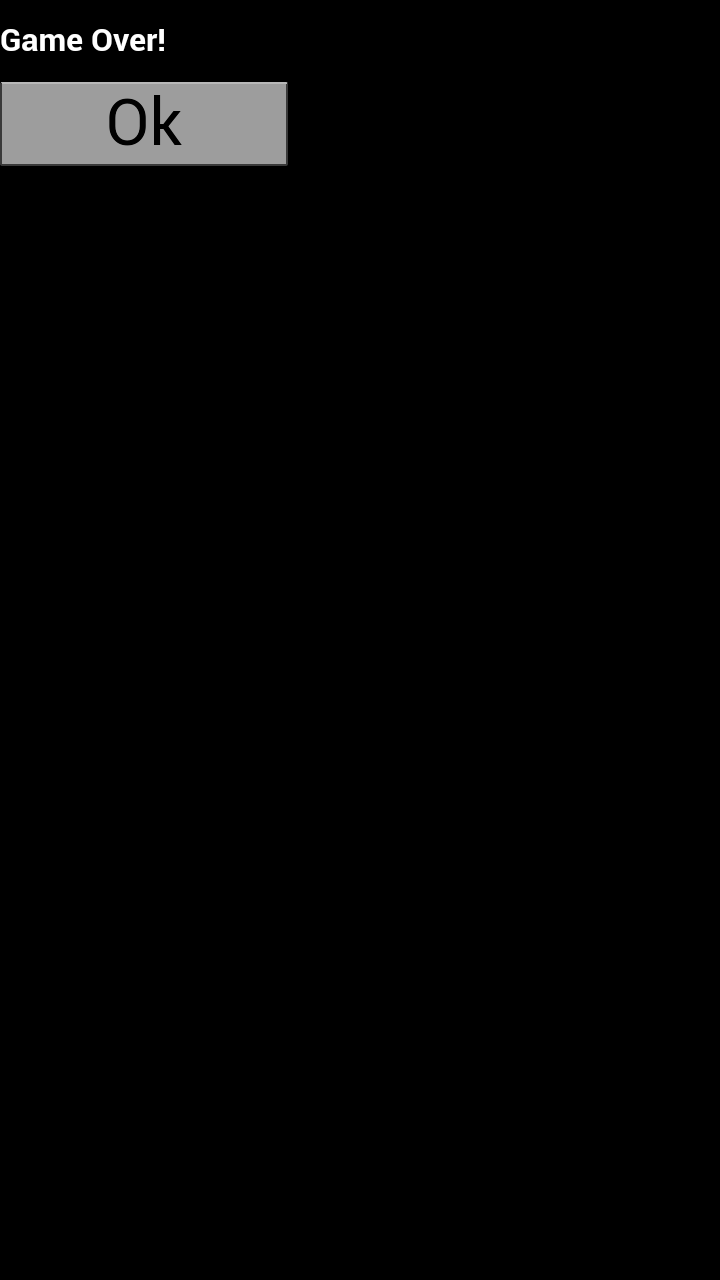
\includegraphics[scale=0.17]{pictures/sprint2-screen/sprint2-10}
	}
	\subfigure{
		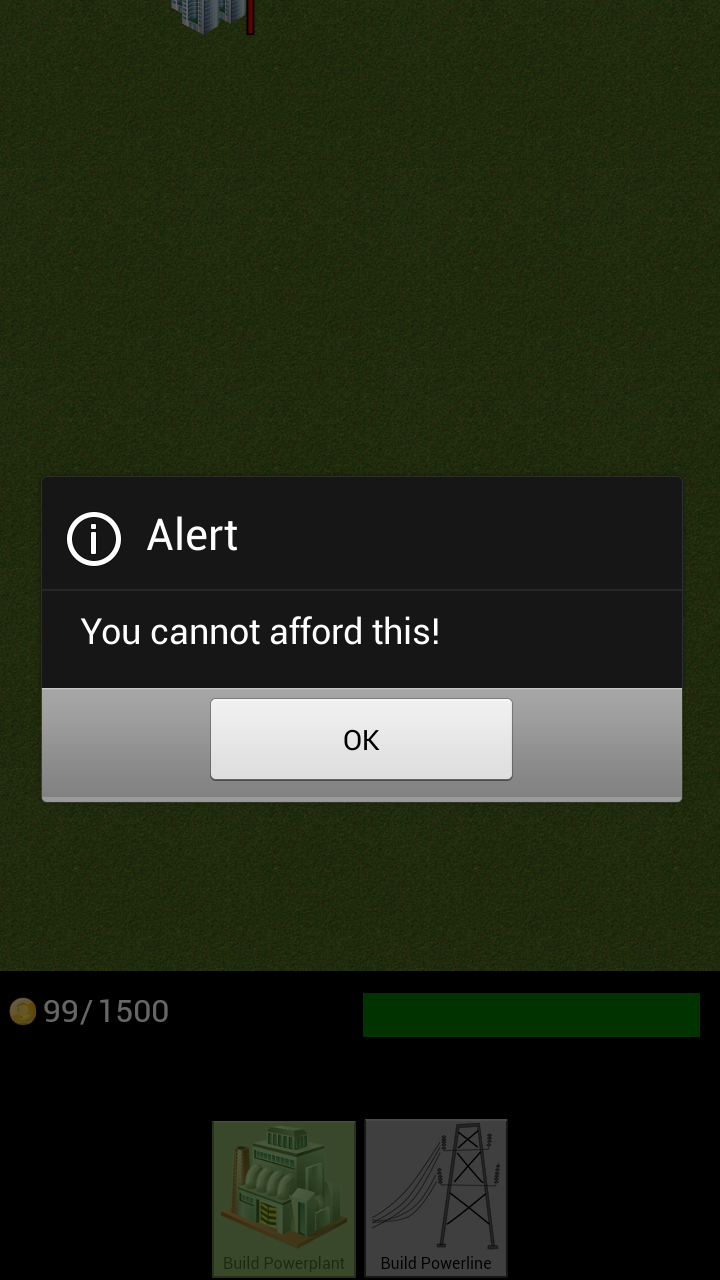
\includegraphics[scale=0.17]{pictures/sprint2-screen/sprint2-11}
	}
	\caption{This is blabla}
	\end{figure}

\clearpage
\subsection{Testing}

	\subsubsection{Tests introduced in this sprint}

	The functional tests executed in this sprint are listed here. The test cases can be found in chapter 7.4.

	\definecolor{lightgray}{gray}{0.9}

	\begin{tabular}{| p{2cm} | p{7cm} | p{3cm} |}
		\hline
		\rowcolor{lightgray}
		{\bf Test Case} & {\bf Result} & {\bf Pass/Not pass} \\ \hline
	  	
	  	FT-04 Main Menu & Works as expected. & Pass. \\ \hline

		FT-05 Build Power Plants & It is still possible to build on top of other buildings, otherwise it works as expected. & Needs minor adjustment. Retest. \\ \hline

		FT-06 Build Power Lines & Building power lines is currently free, it is possible to connect a building to several power plants, and Power lines may cross each other. Otherwise it works as expected. & Needs minor adjustments. Retest. \\ \hline

		FT-07 Information on Buildings and Power Plants & No information on buildings yet. No information on what upgrade does for the Power Plant, but the rest of the information is there. Most of the logic is there. & Retest.\\ \hline

		FT-08 Upgrade Power Plant & Upgrading a power plant cost money and changes the information on the power plant, but does not yet affect the amount the power plant can supply. This will be implemented at a later stage. & Pass. Retest. \\ \hline

		FT-09 Building Mode & Works as expected & Pass. \\ \hline

		FT-10 Tilting & Works as expected & Pass. \\ \hline

		FT-11 Collect Money & Works as expected & Pass. \\ \hline

		FT-12 No Power and Health Bar & Works as expected & Pass. \\ \hline

		FT-13 Game Over & Works as expected. & Pass. \\ \hline

	\end{tabular}

	\subsubsection{Redone tests}

	The following are the tests that has been executed again this sprint, because they did not pass last sprint:

	\begin{tabular}{| p{2cm} | p{7cm} | p{3cm} |}
		\hline
		\rowcolor{lightgray}
		{\bf Test Case} & {\bf Result} & {\bf Pass/Fail} \\ \hline

		FT-02 Appearance of buildings & Buildings appear at a more controlled rate and now has the ability to disappear. But they can appear on top of each other. & Needs some minor adjustments. Retest. \\ \hline

	\end{tabular}

\subsection{Changes to the requirements}
	In this sprint the group have made some changes. Since last sprint meeting, 
	the group hoped that the customer would change, add or remove requirements, 
	but this have not happend. During the implementation in this sprint, the 
	scrum team did come up with changes to the requirements. 
	Some requirements are moved, changed, splitted or removed.
	In the end of sprint 2 we had the version 3 of the requirement specification 
	and here are the changes:


	{\bf Changes on version 1 of the requirement specification:} \\
	\begin{tabular}{| p{1.5cm} | p{12cm} |}
		\hline
		\rowcolor{lightgray}
		{\bf FR} & {\bf Change} \\ \hline
		FR3.3 & {\bf \color{green} [NEW]} There should be several types of buildings on the map, 
		with different power requirements  \\ \hline
		FR3.4 & {\bf \color{green} [NEW]} Different types of building should reward different amounts of 
		money \\ \hline
		FR3.6 & {\bf \color{orange} [CHANGED]}changed priority from high to critical \\ \hline
		FR4.4 & {\bf \color{red} [REMOVED]} As the user reaches higher levels there should be an 
		increase in faulty power cables \\ \hline
		FR5.2 & {\bf \color{red} [REMOVED]} There should be buildings on the map for the user to 
		supply with power; new buildings should appear over time. \\ \hline
		FR5.4 & {\bf \color{red} [REMOVED]} The player should be able to suspend specific buildings' 
		power supply in order to server others \\ \hline
		FR5.5 & {\bf \color{orange} [MOVED TO GUI]} A power preservation tip should appear when the 
		user reaches a new level. \\ \hline
	\end{tabular}

	{\bf Changes on version 2 of the requirement specification:} \\
	\begin{tabular}{| p{1.5cm} | p{12cm} |}
		\hline
		\rowcolor{lightgray}
		{\bf FR} & {\bf Change} \\ \hline
		FR1.9 & {\bf \color{green} [NEW]} There should be played a sound effect when 
		the player collects money \\ \hline
		FR1.10 & {\bf \color{green} [NEW]} There should be played a sound effect when 
		the player upgrades the powerplant \\ \hline
		FR1.11 & {\bf \color{green} [NEW]} There should be played a sound effect when 
		the player builds a power cable \\ \hline
		FR1.12 & {\bf \color{green} [NEW]} The user should not get the oppertunity to 
		tilt the screen by tilting the phone. \\ \hline
		FR2.4 & {\bf \color{orange} [MOVED TO INCOMING/OUTGOING MONEY]} The user should 
		be able to connect the buildings to the powerplants by building a power cable. 
		Building cables costs money. \\ \hline
		FR3.6 & {\bf \color{green} [NEW]} When an existing building is not supplied 
		with power within a certain amount of time, the house should dissapear and the player's 
		health score should decrease \\ \hline
		FR3.6 & {\bf \color{orange} [MOVED TO GUI]} The user should be able to see 
		that a building has gone without power for some time, and is affecting the 
		player's health score if the building is not connected to a powerplant before it 
		dissapears. \\ \hline
		FR4.3 & {\bf \color{orange} [MOVED TO OBSTACLES]} When an existing building 
		is not supplied with power within a certain amount of time, the house should 
		dissapear and the player's health score should decrease \\ \hline
		FR5.4 & {\bf \color{green} [NEW]} The user should be able to upgrade the powerplant. 
		This cost money. \\ \hline
		FR6.7 & {\bf \color{green} [NEW]} The user should be able to see the main 
		menu when he/she starts the game. \\ \hline
		FR6.8 & {\bf \color{green} [NEW]} When the player wants to place a powerplant 
		or a power cable in building mode, the player should be prompted if they want to 
		go through with it, or cancel. \\ \hline
		FR6.9 & {\bf \color{green} [NEW]} The user should be able to see that he/she 
		is in building mode when selecting a building to build in the hub menu. \\ \hline
	\end{tabular}

\subsection{Group dynamics}
	In sprint 1 the group had some problems with the group dynamics. 
	During this sprint we managed to work together as a group and the group dynamics
	is now very good. The changes that helped the group to work better as a group
	was the allocation of roles in the last sprint. 

\subsection{Customer feedback}
	In this sprint the group got a feedback from the customer in the end of the sprint.
	The customer think that we are working structured and the flow of information is good.
	They are very pleased with the cooperation this far in the project.

	After the sprint meeting, the customer tested the game on a phone. The feedback on the game
	was that they had some problems with building the powelines as well as knowing how to play.
	The group will try to solve the problems until the next meeting.

	The customer is also very pleased with the requirement specification and the priorities
	that we have made. So far, the group has implemented the most of the critical and high
	priorities and the requirements left in the backlog is mainly medium/low. 

\subsection{Sprint retrospective}
	\subsubsection*{Start doing: } 
		\begin{itemize}
			\item use branches for new features to be implemented and not implement new 
			features in the master branch.
		\end{itemize}
	\subsubsection*{Stop doing: }

	\subsubsection*{Continue doing: }
		\begin{itemize}
			\item Keep up the good team work
		\end{itemize}

